
% v2-acmsmall-sample.tex, dated March 6 2012
% This is a sample file for ACM small trim journals
%
% Compilation using 'acmsmall.cls' - version 1.3 (March 2012), Aptara Inc.
% (c) 2010 Association for Computing Machinery (ACM)
%
% Questions/Suggestions/Feedback should be addressed to => "acmtexsupport@aptaracorp.com".
% Users can also go through the FAQs available on the journal's submission webpage.
%
% Steps to compile: latex, bibtex, latex latex
%
% For tracking purposes => this is v1.3 - March 2012
\documentclass[prodmode,acmtecs]{acmsmall} % Aptara syntax
\usepackage[spanish,polish]{babel}
\usepackage[T1]{fontenc}
\usepackage{fancyvrb}
\usepackage{graphicx,hyperref}
\newcommand\cutout[1]{}


\usepackage[table]{xcolor}
\usepackage[utf8]{inputenc}
\usepackage[parfill]{parskip}
\usepackage{tabulary}
\PassOptionsToPackage{hyphens}{url}
\usepackage{hyperref}    
\usepackage[capitalize]{cleveref}


% Metadata Information
% !!! TODO: SET THESE VALUES !!!
\acmVolume{0}
\acmNumber{0}
\acmArticle{CFP}
\acmYear{0}
\acmMonth{0}

\newcounter{colstart}
\setcounter{page}{4}

\RecustomVerbatimCommand{\VerbatimInput}{VerbatimInput}%
{
%fontsize=\footnotesize,
fontfamily=\rmdefault
}


\newcommand{\UnderscoreCommands}{%\do\verbatiminput%
\do\citeNP \do\citeA \do\citeANP \do\citeN \do\shortcite%
\do\shortciteNP \do\shortciteA \do\shortciteANP \do\shortciteN%
\do\citeyear \do\citeyearNP%
}

\usepackage[strings]{underscore}



% Document starts
\begin{document}


\setcounter{colstart}{\thepage}

\acmArticle{CFP}
\title{\huge\sc SIGLOG Monthly 222}
\author{DAVID PURSER\affil{Max Planck Institute for Software Systems, Saarbr\"ucken}
\vspace*{-2.6cm}\begin{flushright}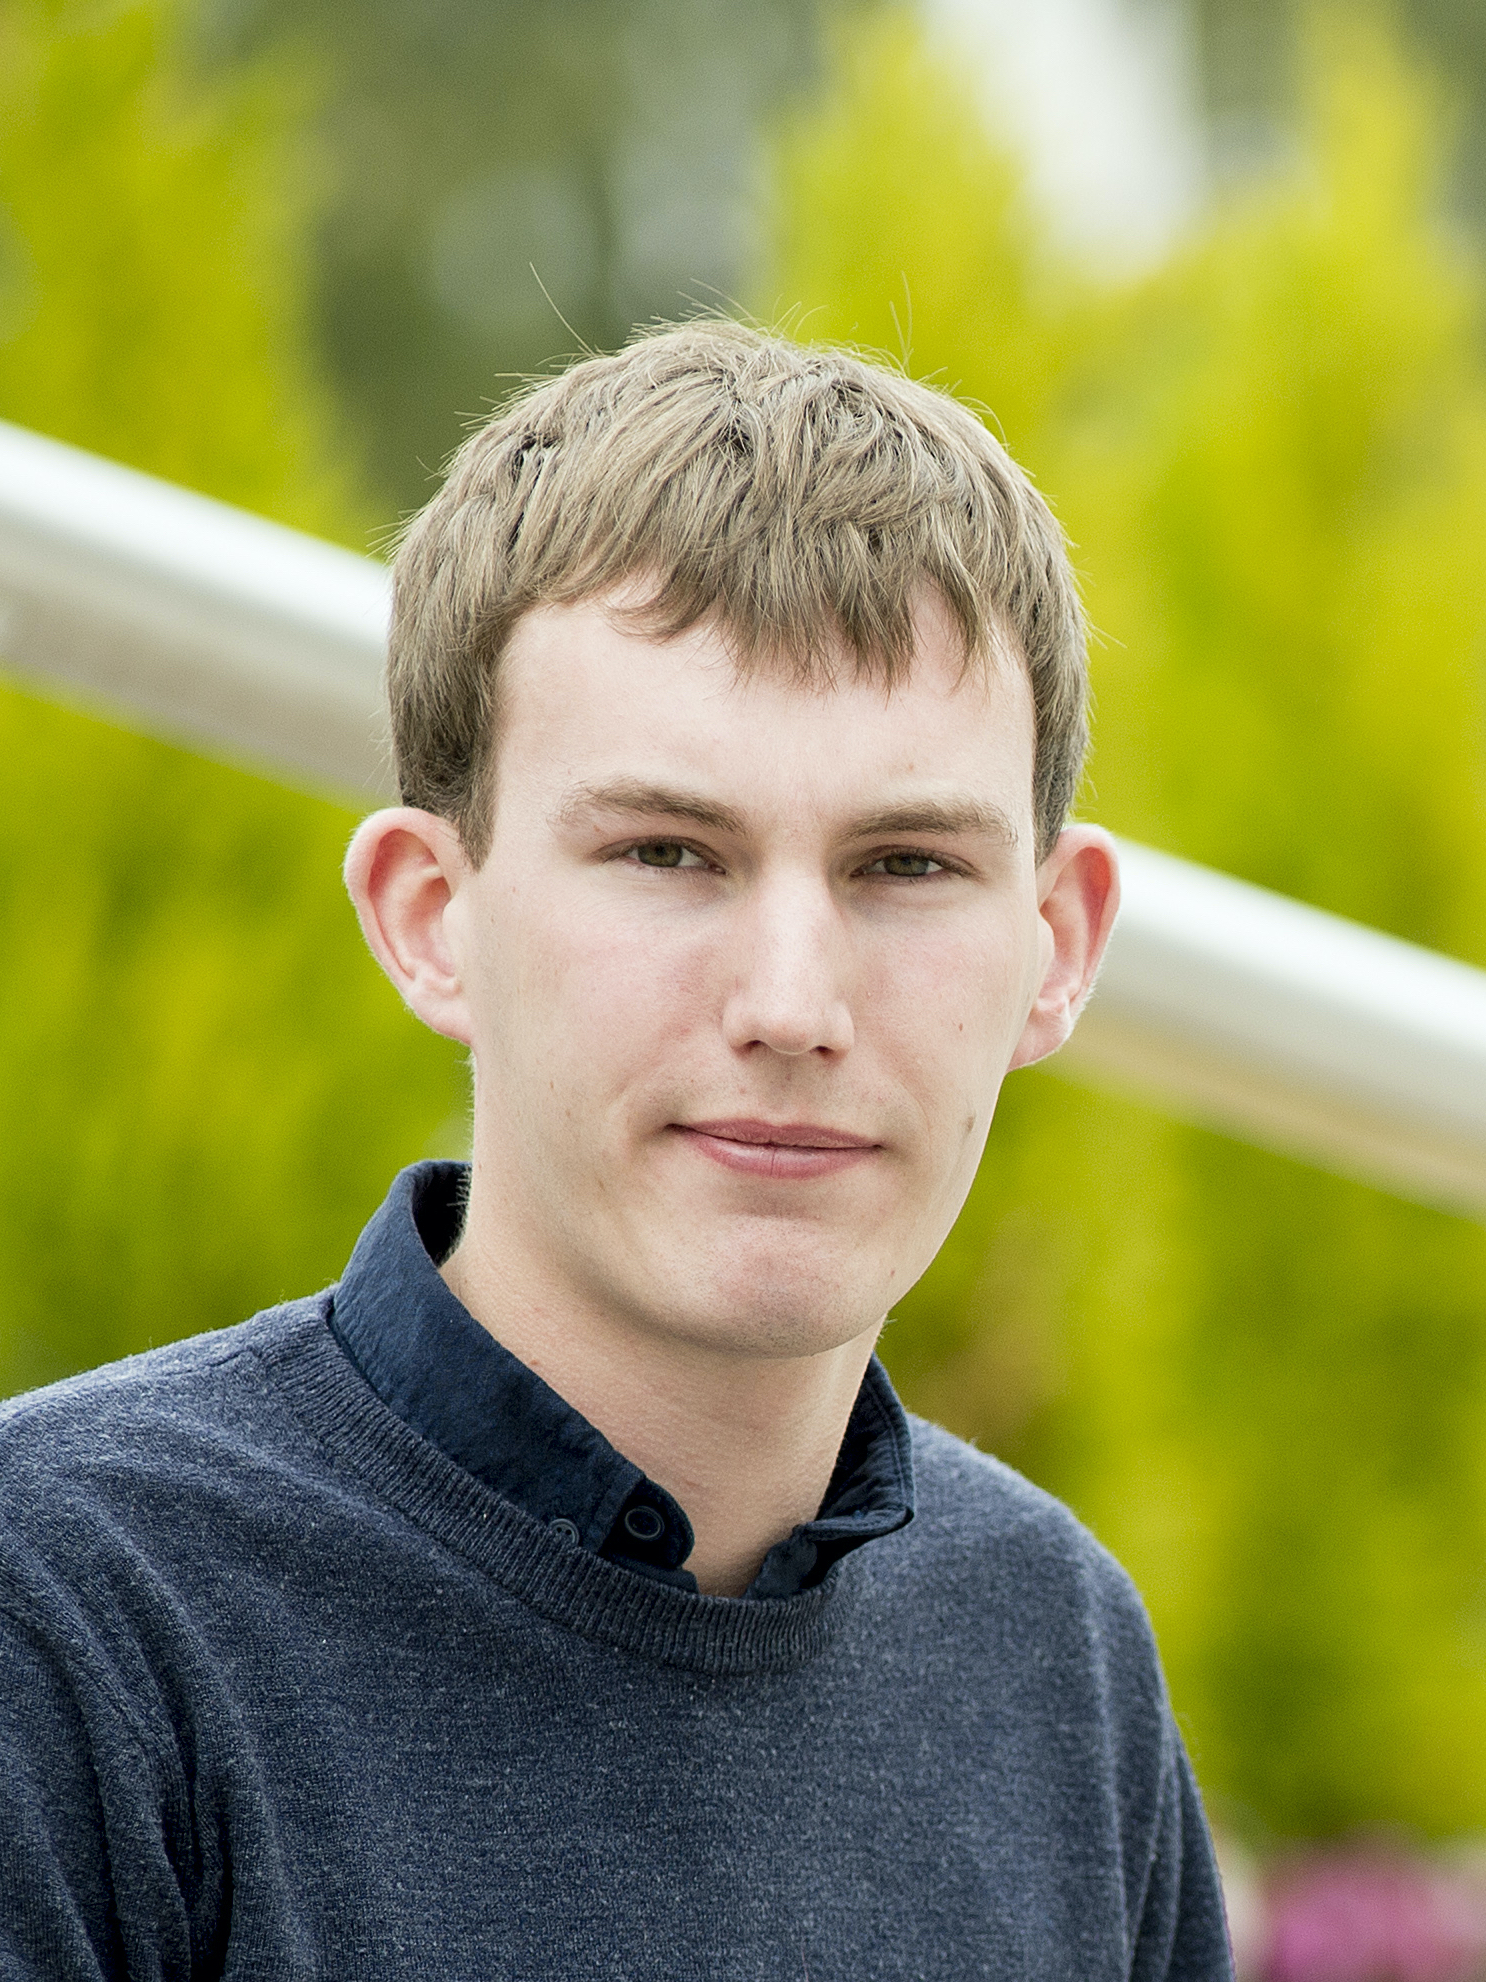
\includegraphics[width=30mm]{dp}\end{flushright}
}

\maketitlee

\href{https://lics.siglog.org/newsletters/}{Past Issues}
 - 
\href{https://lics.siglog.org/newsletters/inst.html}{How to submit an announcement}
\section{Table of Content}\begin{itemize}\item DEADLINES (\cref{deadlines}) 
 
\item SIGLOG MATTERS 
 
\begin{itemize}\item The 2022 Alonzo Church Award for Outstanding Contributions to Logic and Computation (\cref{The2022AlonzoChurchAwardforOutstandingContributionstoLogicandComputation})
\end{itemize} 
\item CALLS 
 
\begin{itemize}\item CSL 22 (CALL FOR PARTICIPATION) (\cref{CSL22})
\item FSCD 2022 (CALL FOR PAPERS) (\cref{FSCD2022})
\item HSCC 2022 (CALL FOR POSTERS AND DEMOS) (\cref{HSCC2022})
\item LPNMR 2022 (CALL FOR WORKSHOPS, CALL FOR PAPER) (\cref{LPNMR2022})
\item Gödel Prize 2022 (CALL FOR NOMINATIONS) (\cref{GdelPrize2022})
\item LearnAut (CALL FOR SUBMISSIONS) (\cref{LearnAut})
\item NALOMA 22 (CALL FOR PAPERS) (\cref{NALOMA22})
\end{itemize} 
\end{itemize}\section{Deadlines}\label{deadlines}\rowcolors{1}{white}{gray!25}\begin{tabulary}{\linewidth}{LL}CSL 2022:  & Feb 06, 2022 (Registration) \\
FSCD 2022:  & Feb 08, 2022 (Abstract), Feb 11, 2022 (Paper) \\
IJCAR 2022:  & Feb 11, 2022 (Paper) \\
HSCC 2022:  & Feb 14, 2022 (Posters and demos) \\
FoIKS 2022:  & Feb 18, 2022 (Abstract, extended), Feb 25, 2022 (Paper, extended) \\
CAV AWARD:  & Feb 20, 2022 (Nomination deadline) \\
ICGT 2022:  & Feb 21, 2022 (Abstract), Feb 28, 2022 (Paper) \\
LPNMR 2022:  & Feb 25, 2022 (Workshop proposals), Apr 23, 2022 (Paper registration), Apr 30, 2022 (Paper) \\
Gödel Prize 2022:  & Feb 28, 2022 (Nominations deadline) \\
AiML 2022:  & Mar 07, 2022 (Abstracts for full papers), Mar 14, 2022 (Full papers), May 23, 2022 (Short presentations) \\
TYPES 2022 and CA20111:  & Mar 09, 2022 (2 page abstract) \\
LearnAut:  & Mar 31, 2022 (Submission deadline) \\
Alonzo Church Award:  & Apr 02, 2022 (Deadline for nominations) \\
NALOMA 22:  & Apr 15, 2022 (Papers \& extended abstracts) \\
FORMATS 2022:  & Apr 19, 2022 (Abstract), Apr 22, 2022 (Paper) \\
ATVA 2022:  & Apr 24, 2022 (Abstract), May 01, 2022 (Paper) \\
\end{tabulary}
\section{The 2022 Alonzo Church Award for Outstanding Contributions to Logic and Computation}\label{The2022AlonzoChurchAwardforOutstandingContributionstoLogicandComputation}CALL FOR NOMINATIONS 

\begin{itemize}\item  INTRODUCTION 
 
  An annual award, called the Alonzo Church Award for Outstanding Contributions to Logic and Computation, was established in 2015 by the ACM Special Interest Group for Logic and Computation (SIGLOG), the European Association for Theoretical Computer Science (EATCS), the European Association for Computer Science Logic (EACSL), and the Kurt Goedel Society (KGS). The award is for an outstanding contribution represented by a paper or by a small group of papers published within the past 25 years. This time span allows the lasting impact and depth of the contribution to have been established. The award can be given to an individual, or to a group of individuals who have collaborated on the research. For the rules governing this award, see \href{https://siglog.org/alonzo-church-award/}{https://siglog.org/alonzo-church-award/}, \href{https://www.eatcs.org/index.php/church-award/}{https://www.eatcs.org/index.php/church-award/}, and \href{https://www.eacsl.org/alonzo-church-award/}{https://www.eacsl.org/alonzo-church-award/}. 
 
  The 2021 Alonzo Church Award was given jointly to Georg Gottlob, Christoph Koch, Reinhard Pichler, Luc Segoufin and Klaus U. Schulz for their ground-breaking work on logic-based web-data extraction, and querying tree-structured data. Lists containing this and all previous winners can be found through the links above.  
 
\item  ELIGIBILITY AND NOMINATIONS 
 
  The contribution must have appeared in a paper or papers published within the past 25 years. Thus, for the 2022 award, the cut-off date is January 1, 1997. When a paper has appeared in a conference and then in a journal, the date of the journal publication will determine the cut-off date. In addition, the contribution must not yet have received recognition via a major award, such as the Turing Award, the Kanellakis Award, or the Goedel Prize. (The nominee(s) may have received such awards for other contributions.) While the contribution can consist of conference or journal papers, journal papers will be given a preference. 
 
  Nominations for the 2022 award are now being solicited. The nominating letter must summarize the contribution and make the case that it is fundamental and outstanding. The nominating letter can have multiple co-signers. Self-nominations are excluded. Nominations must include: a proposed citation (up to 25 words); a succinct (100-250 words) description of the contribution; and a detailed statement (not exceeding four pages) to justify the nomination. Nominations may also be accompanied by supporting letters and other evidence of worthiness. 
 
  Nominations should be submitted to rjagadee@depaul.edu by April 2, 2022. 
 
\item  PRESENTATION OF THE AWARD 
 
  The 2022 award will be presented at the Federated Logic Conference 2022, which is scheduled to take place in Haifa, Israel in July/August 2022. The award will be accompanied by an invited lecture by the award winner, or by one of the award winners. The awardee(s) will receive a certificate and a cash prize of USD 2,000. If there are multiple awardees, this amount will be shared. 
 
\item  AWARD COMMITTEE 
 
  The 2022 Alonzo Church Award Committee consists of the following five members: Thomas Colcombet, Mariangiola Dezani, Javier Esparza, Radha Jagadeesan (chair), and Igor Walukiewicz. 
 
\end{itemize}\section{CSL 22: Computer Science Logic }\label{CSL22}  Online, Feb 14-19, 2022, hosted by the University of Göttingen\\ 
  \href{http://csl2022.uni-goettingen.de/}{http://csl2022.uni-goettingen.de/}\\ 
CALL FOR PARTICIPATION 

  News: Online conference; Registration is open; List of accepted papers; Ackermann awards. \\ 
\begin{itemize}\item  Computer Science Logic (CSL) is the annual conference of the European Association for Computer Science Logic (EACSL), see \href{https://www.eacsl.org/}{https://www.eacsl.org/}.  CSL is an interdisciplinary conference, spanning across both basic and application oriented research in mathematical logic and computer science.   
 
\item  INVITED SPEAKERS 
 
\begin{itemize}\item  Annabelle McIver Macquarie (University, Sydney, Australia)
\item  Udi Boker (IDC Herzliya, Israel)
\item  Martin Escardo (University of Birmingham, UK)
\item  Rosalie Iemhoff (Utrecht University, The Netherlands)
\item  Karen Lange (Wellesley College, USA)
\end{itemize} 
\item  ACCEPTED PAPERS 
 
  \href{http://csl2022.uni-goettingen.de/#acceptedpaper}{http://csl2022.uni-goettingen.de/\#acceptedpaper} 
 
\item  REGISTRATION 
 
  Registration form: \href{https://events.gwdg.de/event/95/}{https://events.gwdg.de/event/95/} 
 
  The participation fee for CSL 2022 is as follows: 
 
\begin{itemize}\item  members of EACSL (2022): free
\item  students: 5 Euro
\item  members of EATCS or ACM SIGLOG (2022): 15 Euro
\item  regular: 20 Euro  
\end{itemize} 
  This fee covers participation in CSL 2022 and includes membership of EACSL for 2022 (\href{https://www.eacsl.org/membership/}{https://www.eacsl.org/membership/}). This fee has to be paid directly to the EACSL, as indicated in the registration process, and is processed by the EACSL. 
 
  There is no participation fee for the collocated workshops (see below), and they can be attended without paying the CSL registration fee, but the CSL-registration form should still be filled. 
 
  These participation fees are made possible only due to the generous financial support by the German Research Foundation (DFG) and the University of Göttingen. 
 
\item  IMPORTANT DATES 
 
  All participants must register. 
 
Non-speaker registration deadline: Feb 06, 2022 
 
\item  Helena-Rasiowa-Award 
 
  The Helena Rasiowa Award is the best student paper award for the CSL conference series, starting from CSL 2022. The award will be given to the best paper (as decided by the PC) written solely by students or for which students were the main contributors. The Helena-Rasiowa-Award will be announced during the conference. 
 
  Read more about the contribution of Helena Rasiowa to logic and computer science, and their interplay, here: \href{https://www.eacsl.org/?page_id=1104}{https://www.eacsl.org/?page\_id=1104} 
 
\item  Ackermann Award 2021 
 
  The Ackermann Award is the EACSL Outstanding Dissertation Award for Logic in Computer Science. The award for 2021 will be presented during CSL 2022. 
 
  The Ackermann Award 2021 is given to two PhD theses (in alphabetic order): 
 
\begin{itemize}\item  Marie Fortin for her thesis ``Expressivity of first-order logic, star-free propositional dynamic logic and communicating automata'' defended at ENS Paris-Saclay, (France) in 2020. Supervisors: Paul Gastin and Benedikt Bollig
\item  Sandra Kiefer for her thesis ``Power and Limits of the Weisfeiler-Leman Algorithm'' defended at RWTH Aachen, (Germany) in 2020. Examiners: Martin Grohe, Pascal Schweitzer, Neil Immerman
\end{itemize} 
\item  COLOCATED EVENTS 
 
\begin{itemize}\item  LCC 2022: Logic and Computational Complexity
\end{itemize} 
    Meetings of the workshop ``Logic and Computational Complexity'' are aimed at the foundational interconnections between logic and computational complexity, as present, for example, in implicit computational complexity (descriptive and type-theoretic methods); deductive formalisms as they relate to complexity (e.g. ramification, weak comprehension, bounded arithmetic, linear logic and resource logics); complexity aspects of finite model theory and databases; complexity-mindful program derivation and verification; computational complexity at higher type; and proof complexity. LCC 2022 will be the 23rd workshop in the series, see \href{https://www.cs.swansea.ac.uk/lcc/}{https://www.cs.swansea.ac.uk/lcc/}. The program will consist of invited lectures as well as contributed papers selected by the Program Committee. 
 
\begin{itemize}\item  LMW@CSL: Logic Mentoring Workshop
\end{itemize} 
    The Logic Mentoring Workshop introduces young researchers to the technical and practical aspects of a career in logic research. It is targeted at students, from senior undergraduates to graduates, and will include talks and panel sessions from leaders in the subject. Building on successful LMW editions from past years, its first winter edition will be collocated with CSL 2022. Website: \href{https://lmw.mpi-sws.org/csl/}{https://lmw.mpi-sws.org/csl/} 
 
\end{itemize}\section{FSCD 2022: Seventh International Conference on Formal Structures for Computation and Deduction }\label{FSCD2022}  August 2 - 5, 2022, Haifa, Israel\\ 
  \href{https://fscd2022.github.io}{https://fscd2022.github.io}\\ 
  In-cooperation with ACM SIGLOG and SIGPLAN\\ 
CALL FOR PAPERS 

\begin{itemize}\item  IMPORTANT DATES (AoE) 
 
\rowcolors{1}{white}{gray!25}\begin{tabulary}{\linewidth}{LL}Abstract submission:  & Feb 08, 2022 \\
Paper submission:  & Feb 11, 2022 \\
Rebuttal:  & Mar 29-Apr 1, 2022 \\
Notification:  & Apr 15, 2022 \\
Final version:  & Apr 30, 2022 \\
\end{tabulary}
 
\item  INVITED SPEAKERS 
 
\begin{itemize}\item  Cynthia Kop, Radboud University Nijmegen (FSCD Invited Speaker)
\item  Alwen Tiu, The Australian National University (FSCD Invited Speaker)
\item  Orna Kupferman, Hebrew University (FLoC Plenary Speaker)
\item  Catuscia Palamidessi, INRIA Saclay and LIX (FLoC Keynote Speaker)
\end{itemize} 
\item  AFFILIATED WORKSHOPS   
 
\begin{itemize}\item  IFIP-WG1.6: Annual Meeting of the IFIP Working Group 1.6 on Term Rewriting (July 31, only invited talks)  
\item  HoTT/UF: 7th Workshop on Homotopy Type Theory/Univalent Foundations (July 31-August 1)  
\item  IWC: 11th International Workshop on Confluence (August 1)  
\item  LFMTP: International Workshop on Logical Frameworks and Meta-Languages: Theory and Practice (August 1)  
\item  Linearity-TLLA: 3rd Joint International Workshop (July 31-August 1)  
\item  TERMGRAPH: 12th International Workshop on Computing with Terms and Graphs (August 1)  
\item  WiL: 6th Workshop on Women in Logic (July 31)  
\item  WPTE: 9th International Workshop on Rewriting Techniques for Program Transformations and Evaluation (July 31)
\end{itemize} 
\item  OVERVIEW 
 
  FSCD covers all aspects of formal structures for computation and deduction from theoretical foundations to applications. Building on two communities, RTA (Rewriting Techniques and Applications) and TLCA (Typed Lambda Calculi and Applications), FSCD embraces their core topics and broadens their scope to closely related areas in logics, models of computation, semantics and verification in new challenging areas. 
 
\item  TOPICS  
 
  The suggested, but not exclusive, list of topics for submission is: 
 
\begin{itemize}\item  Calculi: Rewriting systems (string, term, higher-order, graph, conditional, modulo, infinitary, etc.); Lambda calculus; Logics (first-order, higher-order, equational, modal, linear, classical, constructive, etc.); Proof theory (natural deduction, sequent calculus, proof nets, etc.); Type theory and logical frameworks; Homotopy type theory; Quantum calculi.
\item  Methods in Computation and Deduction: Type systems (polymorphism, dependent, recursive, intersection, session, etc.); Induction, coinduction; Matching, unification, completion, orderings; Strategies (normalization, completeness, etc.); Tree automata; Model building and model checking; Proof search and theorem proving; Constraint solving and decision procedures.
\item  Semantics: Operational semantics and abstract machines; Game Semantics and applications; Domain theory and categorical models; Quantitative models (timing, probabilities, etc.); Quantum computation and emerging models in computation.
\item  Algorithmic Analysis and Transformations of Formal Systems: Type Inference and type checking; Abstract Interpretation; Complexity analysis and implicit computational complexity; Checking termination, confluence, derivational complexity and related properties; Symbolic computation.
\item  Tools and Applications: Programming and proof environments; Verification tools; Proof assistants and interactive theorem provers; Applications in industry; Applications of formal systems in other sciences.
\item  Semantics and Verification in new challenging areas: Certification; Security; Blockchain protocols; Data Bases; Deep learning and machine learning algorithms; Planning.
\end{itemize} 
\item  SUBMISSION GUIDELINES 
 
  Papers must be submitted, in LIPIcs format, to: \href{https://easychair.org/conferences/?conf=fscd2022}{https://easychair.org/conferences/?conf=fscd2022} 
 
  Submissions can be made in two categories.  Regular research papers are limited to 15 pages, excluding references and appendices.  They must present original research which is unpublished and not submitted elsewhere.  System descriptions are limited to 15 pages, excluding references.  They must present new software tools, or significantly new versions of such tools, in which FSCD topics play an important role. An archive of the code with instructions on how to install and run the tool must be submitted.  In addition, a webpage where the system can be experimented with should be provided. 
 
  One author of an accepted paper is expected to present it at the (physical) conference, unless Covid restrictions prevent travel. 
 
  Authors of selected papers will be invited to submit an extended version to a special issue of Logical Methods in Computer Science. 
 
\item  BEST PAPER AWARD BY JUNIOR RESEARCHERS 
 
  The program committee will select a paper in which at least one author is a junior researcher, i.e. either a student or whose PhD award date is less than three years from the first day of the meeting. Other authors should declare to the PC Chair that at least 50% of contribution is made by the junior researcher(s). 
 
\end{itemize}\section{HSCC 2022: 25th ACM International Conference on Hybrid Systems: Computation and Control}\label{HSCC2022}  Part of CPS-IoT Week 2022\\ 
  May 4-6, 2022, Milan, Italy\\ 
  \href{https://hscc.acm.org/2022/}{https://hscc.acm.org/2022/}\\ 
CALL FOR POSTERS AND DEMOS 

\begin{itemize}\item  Scope of HSCC 
 
  Hybrid Systems: Computation and Control (HSCC) 2022 is the 25th in a series of conferences focusing on original research on concepts, tools, and techniques from computer science, control theory, and applied mathematics for the analysis and control of hybrid dynamical systems with an emphasis on computational aspects. By drawing on strategies from computation and control, the hybrid systems field offers techniques that are applicable to both man-made cyber-physical systems (ranging from small robots to global infrastructure networks) and natural systems (ranging from biochemical networks to physiological models). The conference covers a wide spectrum of topics from theoretical results to practical considerations, and from academic research to industrial adoption. 
 
\item  Posters and Demos 
 
  Posters presented at the conference will provide an opportunity for conference attendees to interact with researchers in an informal setting. Posters may be about already accepted papers, ongoing research projects, discussions on new problem statements, or preview of late-breaking results. Demos will give the audience a closer look at tools and techniques, and offer an interactive experience with the demonstrated entities. 
 
  The selection criteria for acceptance will be: novelty, technical merit, relevance to HSCC and, especially for demos, details on the presentation. If desired and not previously published, abstracts up to 2 page in length describing the poster or demo will be included for publication in the electronic proceedings of HSCC.   
 
  These sessions are an excellent way to exchange ideas and for presenters to obtain feedback from the attendees. 
 
  A Best Poster/Demo prize will be awarded and announced during the conference and on the website. 
 
  See \href{https://hscc.acm.org/2022/call-for-posters-and-demos/}{https://hscc.acm.org/2022/call-for-posters-and-demos/} for more information and submission instructions. 
 
\item  Deadline: Feb 14, 2022  AOE 
 
\end{itemize}\section{LPNMR 2022: 16th International Conference on Logic Programming and Non-monotonic Reasoning  }\label{LPNMR2022}  \href{https://sites.google.com/view/lpnmr2022}{https://sites.google.com/view/lpnmr2022} \\ 
  Genova, Italy\\ 
  September 5-8, 2022\\ 
\begin{itemize}\item  AIMS AND SCOPE 
 
  LPNMR 2022 is the sixteenth in the series of international meetings on logic programming and non-monotonic reasoning. LPNMR is a forum for exchanging ideas on declarative logic programming, non-monotonic reasoning, and knowledge representation. The aim of the conference is to facilitate interactions between researchers and practitioners interested in the design and implementation of logic-based programming languages and database systems, and those working in knowledge representation and non-monotonic reasoning. LPNMR strives to encompass theoretical and experimental studies that have led or will lead to advances in declarative programming and knowledge representation, as well as their use in practical applications. A Doctoral Consortium will also be a part of the program. 
 
  LPNMR 2022 aims to bring together researchers from LPNMR core areas and application areas of the aforementioned kind in order to share research experiences, promote collaboration and identify directions for joint future research.  
 
\end{itemize}CALL FOR WORKSHOPS 

  The objective of the LPNMR workshop program is to stimulate the discussion and the exchange of ideas on topics related, but not limited, to declarative logic programming, non-monotonic reasoning, and knowledge representation. We aim at creating a forum where researchers from a broad spectrum of disciplines may interact and have an opportunity to promote collaboration and identify directions for joint future research. Accordingly, we solicit workshop proposals on theoretical and applied research topics.\\ 
  Workshop proposals should explain and motivate the topic of the workshop, and discuss the format of presentation of the contributes. Workshops will likely be half-day or one-day in duration, but we may consider longer programs. \\ 
\begin{itemize}\item  DATES 
 
\rowcolors{1}{white}{gray!25}\begin{tabulary}{\linewidth}{LL}Workshop proposals submission:  & Feb 25, 2022 \\
Workshop proposals notifications:  & Mar 07, 2022 \\
Workshop program (tentative date):  & Sep 05, 2022 \\
\end{tabulary}
 
\item  SUBMISSION 
 
  \href{https://easychair.org/my/conference?conf=lpnmrws2022}{https://easychair.org/my/conference?conf=lpnmrws2022} 
 
  Proposals should clearly specify the following: 
 
\begin{itemize}\item  Workshop title and acronym
\item  A brief description, emphasizing why this workshop would appeal to
\end{itemize} 
     audiences from LPNMR 
 
\begin{itemize}\item  A list of organizers with email addresses, web page URLs, and a short 
\end{itemize} 
     description of their experience in organizing events 
 
\begin{itemize}\item  A short description of the format of planned activities (talks, posters,
\end{itemize} 
     panels, invited speakers if any, etc.) 
 
\begin{itemize}\item  The proposed duration (half day, one day, etc.)
\item  A description of the history of the workshop (if any)
\item  Expected number of participants
\end{itemize} 
\end{itemize}CALL FOR PAPER 

\begin{itemize}\item  TOPICS 
 
  Authors are invited to submit papers presenting original and unpublished research on all aspects of non-monotonic approaches in logic programming and knowledge representation. We invite submissions of both long and short papers on topics detailed below. 
 
  Conference topics include, but are not limited to: 
 
\begin{itemize}\item  Foundations of LPNMR Systems: Semantics of new and existing languages; Action languages, causality; Formalization of Commonsense Reasoning and understanding its laws and nature; Relationships among formalisms; Complexity and expressive power; Inference algorithms and heuristics for LPNMR systems; Extensions of traditional LPNMR languages such as new logical connectives or new inference capabilities; Updates, revision, and other operations on LPNMR systems; Uncertainty in LPNMR systems.
\item  Implementation of LPNMR systems: System descriptions, comparisons, evaluations; Algorithms and novel techniques for efficient evaluation; LPNMR benchmarks.
\item  Applications of LPNMR: Use of LPNMR in Commonsense Reasoning and other areas of KR; LPNMR languages and algorithms in planning, diagnosis, argumentation, reasoning with preferences, decision making and policies; Applications of LPNMR languages in data integration and exchange systems, software engineering and model checking; Applications of LPNMR to bioinformatics, linguistics, psychology, and other sciences; Integration of LPNMR systems with other computational paradigms; Embedded LPNMR: Systems using LPNMR subsystems. 
\end{itemize} 
\item  SUBMISSION AND PUBLICATION 
 
  LPNMR 2022 welcomes submissions of long papers (13 pages) or short papers (6 pages) in the following categories: 
 
\begin{itemize}\item  Technical papers 
\item  System descriptions 
\item  Application descriptions
\end{itemize} 
  The indicated number of pages includes title page, references and figures. All submissions will be peer-reviewed and accepted papers will appear in the conference proceedings published in the Springer's Lecture Notes in Artificial Intelligence (LNAI) series. At least one author of each accepted paper is expected to register for the conference to present the work. Submissions must be in English, original research, Springer format, not submitted for publication elsewhere, and submitted at \href{https://easychair.org/conferences/?conf=lpnmr2022}{https://easychair.org/conferences/?conf=lpnmr2022} 
 
  The two best papers of general AI interest will be invited for rapid publication in the Artificial Intelligence Journal. 
 
  Also, the 2-5 best papers with a logic programming focus will be invited for rapid publication in the journal of Theory and Practice of Logic Programming.  
 
\item  LPNMR DOCTORAL CONSORTIUM  
 
  A mentoring event where PhD students have a chance to present their current research, get feedback from peers and senior researchers, and establish contacts for their future career.  
 
\item  IMPORTANT DATES 
 
\rowcolors{1}{white}{gray!25}\begin{tabulary}{\linewidth}{LL}Paper registration:  & Apr 23, 2022 \\
Paper submission:  & Apr 30, 2022 \\
Notification:  & Jun 10, 2022 \\
Final versions due:  & Jun 30, 2022 \\
\end{tabulary}
 
\item  VENUE  
 
  The main conference will take place in Genova Nervi, Italy (subject to the pandemic requiring hybrid or online). See website for further details.  
 
\end{itemize}\section{Gödel Prize 2022}\label{GdelPrize2022}CALL FOR NOMINATIONS 

\begin{itemize}\item  The  Gödel Prize for outstanding papers in the area of theoretical computer science is sponsored jointly by the European Association for Theoretical Computer Science (EATCS) and the Special Interest Group on Algorithms and Computation Theory of the Association for Computing Machinery (ACM SIGACT). This award is presented annually. The 30th Gödel Prize will be awarded at the 49th International Colloquium on Automata, Languages and Programming (ICALP). 
 
\item  DEADLINE 
 
  Call for Nominations is now open. 
 
Nominations deadline: Feb 28, 2022 
 
\item  For details, see \href{https://sigact.org/prizes/g%C3%B6del.html}{https://sigact.org/prizes/gödel.html} 
 
\end{itemize}\section{LearnAut: Learning and Automata }\label{LearnAut}  ICALP 2022 workshop\\ 
  July 4th - Paris, France and virtually\\ 
  \href{https://learnaut22.github.io}{https://learnaut22.github.io}\\ 
CALL FOR SUBMISSIONS 

\begin{itemize}\item  Learning models defining recursive computations, like automata and formal grammars, are the core of the field called Grammatical Inference (GI). The expressive power of these models and the complexity of the associated computational problems are major research topics within mathematical logic and computer science. Historically, there has been little interaction between the GI and ICALP communities, though recently some important results started to bridge the gap between both worlds, including applications of learning to formal verification and model checking, and (co-)algebraic formulations of automata and grammar learning algorithms. 
 
  The goal of this workshop is to bring together experts on logic who could benefit from grammatical inference tools, and researchers in grammatical inference who could find in logic and verification new fruitful applications for their methods. 
 
  We invite submissions of recent work, including preliminary research, related to the theme of the workshop. The Program Committee will select a subset of the abstracts for oral presentation. At least one author of each accepted abstract is expected to represent it at the workshop (in person, or virtually).  
 
  Note that accepted papers will be made available on the workshop website but will not be part of formal proceedings (i.e., LearnAut is a non-archival workshop). 
 
\item  TOPICS of interest include (but are not limited to): 
 
\begin{itemize}\item  Computational complexity of learning problems involving automata and formal languages.
\item  Algorithms and frameworks for learning models representing language classes inside and outside the Chomsky hierarchy, including tree and graph grammars.
\item  Learning problems involving models with additional structure, including numeric weights, inputs/outputs such as transducers, register automata, timed automata, Markov reward and decision processes, and semi-hidden Markov models.
\item  Logical and relational aspects of learning and grammatical inference.
\item  Theoretical studies of learnable classes of languages/representations.
\item  Relations between automata or any other models from language theory and deep learning models for sequential data.
\item  Active learning of finite state machines and formal languages.
\item  Methods for estimating probability distributions over strings, trees, graphs, or any data used as input for symbolic models.
\item  Applications of learning to formal verification and (statistical) model checking.
\item  Metrics and other error measures between automata or formal languages.
\end{itemize} 
\item  SUBMISSION INSTRUCTIONS 
 
  Submissions in the form of extended abstracts must be at most 8 single-column pages long at most (plus at most four for bibliography and possible appendixes) and must be submitted in the JMLR/PMLR format.  \href{https://easychair.org/conferences/?conf=learnaut2022}{https://easychair.org/conferences/?conf=learnaut2022}   
 
  We do accept submissions of work recently published or currently under review. 
 
\item  DATES 
 
\rowcolors{1}{white}{gray!25}\begin{tabulary}{\linewidth}{LL}Submission deadline:  & Mar 31, 2022 \\
Notification of acceptance:  & Apr 30, 2022 \\
Early registration:  & TBD \\
\end{tabulary}
 
\end{itemize}\section{NALOMA 22:  Natural Logic Meets Machine Leaning III}\label{NALOMA22}  August 8-18, 2022, during ESSLLI 2022\\ 
  National University of Ireland Galway (hybrid)\\ 
  \href{https://sites.google.com/view/naloma22/home}{https://sites.google.com/view/naloma22/home}\\ 
CALL FOR PAPERS 

\begin{itemize}\item  After the successful completion of NALOMA’20 and NALOMA’21, NALOMA'22 seeks to continue the series and attract exciting contributions. Particularly, this year NALOMA expands its focus to the whole field of Natural Language Understanding (NLU) . The workshop aims to bridge the gap between ML/DL and symbolic/logic-based approaches to NLU and lay a focus on hybrid approaches. NALOMA'22 will take place August 8-18, 2022, during ESSLLI 2022 organized at the National University of Ireland Galway (a hybrid format is planned). 
 
  This workshop invites submissions on any (theoretical or computational) aspect of hybrid methods in any subfield of NLU, including but not limited to NLI, QA, Sentiment Analysis, Dialog, Machine Translation, Summarization, etc. The topics include but are not limited to: 
 
\begin{itemize}\item  hybrid NLU systems that integrate logic-based/symbolic methods with neural networks
\item  explainable NLU models
\item  opening the black-box of deep learning in NLU
\item  downstream hybrid NLU applications
\item  probabilistic semantics for NLU
\item  comparison and contrast between symbolic and deep learning work on NLU
\item  creation, evaluation, and criticism of NLU datasets and how hybrid methods can be used for data cleaning and augmentation
\item  comparison and contrast between human-level and machine-level work in NLU
\item  theoretical notions and necessary refinements of the NLU tasks to address inherent human disagreements
\end{itemize} 
\item  SUBMISSION 
 
  We invite two types of submission: 
 
\begin{itemize}\item  Archival (long or short) papers should report on complete, original and unpublished research. Accepted papers will be published in the workshop proceedings and appear in the ACL anthology. The workshop is endorsed by SIGSEM.
\item  Extended abstracts may report on work in progress or work that was recently published/accepted at a different venue. Extended abstracts will not be included in the workshop proceedings. Thus, the unpublished work will retain the status and can be submitted to another venue. This webpage will link to the accepted extended abstracts. 
\end{itemize} 
  Both accepted papers and extended abstracts are expected to be presented at the workshop. Extended abstracts will be presented as talks or posters at the discretion of the program committee. 
 
  Authors must submit anonymized extended abstracts or papers by April 15. All submissions must adhere to the ACL Guidelines and formatted with ACL style-files or the ACL Overleaf template.  The extended abstracts should not contain an abstract section and may consist of up to 2 pages of content, plus unlimited references. Short and long papers may consist of up to 4 and 8 pages of content, respectively, plus unlimited references. Camera-ready versions of papers will be given one additional page of content so that reviewers’ comments can be taken into account.  
 
  Both extended abstracts and follow-up papers should be submitted via SoftConf (link coming soon). 
 
\item  DATES 
 
\rowcolors{1}{white}{gray!25}\begin{tabulary}{\linewidth}{LL}Papers \& extended abstracts submission:  & Apr 15, 2022 \\
Notification:  & May 25, 2022 \\
Final versions due:  & Jun 15, 2022 \\
Workshop:  & Aug 8-12, 2022 \\
\end{tabulary}
 
\end{itemize}


To the \href{http://siglog.org/}{SIGLOG} or \href{https://lics.siglog.org}{LICS} website\end{document}